% CVPR 2026 Paper Template; see https://github.com/cvpr-org/author-kit

\documentclass[10pt,twocolumn,letterpaper]{article}

%%%%%%%%% PAPER TYPE
% \usepackage[review]{cvpr}      % REVIEW version (anonymous, line numbers)
\usepackage[pagenumbers]{cvpr}   % Course report: named author, page numbers

% Import additional packages in the preamble file, before hyperref
%% This file contains a number of tweaks that are typically applied to the main document.
%% They are not enabled by default, but can be enabled by uncommenting the relevant lines.

%%
%% Inline annotations; for predefined colors, refer to "dvipsnames" in the xcolor package:
%% https://tinyurl.com/overleaf-colors
%%
\newcommand{\red}[1]{{\color{red}#1}}
\newcommand{\todo}[1]{{\color{red}#1}}
\newcommand{\TODO}[1]{\textbf{\color{red}[TODO: #1]}}
%%
%% disable for camera ready / submission by uncommenting these lines  
%%
% \renewcommand{\TODO}[1]{}
% \renewcommand{\todo}[1]{#1}

%%
%% work harder in optimizing text layout. Typically shrinks text by 1/6 of page, enable
%% it at the very end of the writing process, when you are just above the page limit
%%
% \usepackage{microtype}

%%
%% fine-tune paragraph spacing
%%
% \renewcommand{\paragraph}[1]{\vspace{.5em}\noindent\textbf{#1.}}

%%
%% globally adjusts space between figure and caption
%%
% \setlength{\abovecaptionskip}{.5em}


%%
%% Allows "the use of \paper to refer to the project name"
%% with automatic management of space at the end of the word
%%
% \usepackage{xspace}
% \newcommand{\paper}{ProjectName\xspace}

%%
%% Commonly used math definitions
%%
% \DeclareMathOperator*{\argmin}{arg\,min}
% \DeclareMathOperator*{\argmax}{arg\,max}

%%
%% Tigthen underline
%%
% \usepackage{soul}
% \setuldepth{foobar}
\usepackage{booktabs}
\usepackage{tikz}
\usepackage{listings}  % prompts in the appendix
\lstset{basicstyle=\scriptsize\ttfamily, breaklines=true, columns=fullflexible, keepspaces=true}
\usetikzlibrary{arrows.meta,positioning,calc}

\definecolor{cvprblue}{rgb}{0.21,0.49,0.74}
\usepackage[pagebackref,breaklinks,colorlinks,allcolors=cvprblue]{hyperref}

\def\paperID{*****}
\def\confName{CVPR}
\def\confYear{2026}

% TODO: working title
\title{Text to Printable Parts: Which Knowledge Helps an LLM Write, Check and Repair CAD Code?\\
{\large CAP 6938 (AI Knowledge Systems), Fall 2026 --- Final Report}}

\author{Michael Laager\\
University of Central Florida\\
{\tt\small mi740165@ucf.edu}
}

\begin{document}
\maketitle
\begin{abstract}
% One paragraph, ~200 words. Order: task -> system -> what was measured -> headline results -> takeaway.
%  - Task: a chat request in plain words -> a printable STL. The LLM writes CadQuery code; it is run in a sandbox,
%    checked as a mesh and against its stated size, and repaired with the error fed back.
%  - Out of scope for code: organic shapes (sculpted with signed distance functions) or a Thingiverse download.
%  - Round: 7 builder models (2 Claude, 2 Google API, 3 local incl. a fine-tuned 4B) + Thingiverse,
%    48 mechanical + 30 organic cases x 3 runs; right size measured, right shape by a visual judge chosen on
%    146 blind hand grades.
%  - Headline (report-v1.md, Summary): right size + shape Sonnet 99%, Haiku 94%, Gemini Flash Lite 74%,
%    local gemma4:12b 55%, fine-tuned Qwen 4B 30% (base 13%).
%  - Knowledge findings: retrieved examples don't help API models (74% vs 74%) but help the fine-tuned 4B
%    (+12 pts); the repair loop lifts mid-strength models (Gemini 67% -> 88% correct) and sculpting depends on it;
%    sculpting (Haiku 82%) beats Thingiverse downloads (37%) on organic shapes.
\TODO{abstract}
\end{abstract}

\section{Introduction}
\label{sec:intro}

% Motivation (1 paragraph): 3D printers are common, CAD skills are not. Text-to-3D mesh models make shapes that
% look right but have no exact dimensions, holes or wall thicknesses. Parametric CAD code is a better output for an
% LLM: exact, editable, and checkable by running it and measuring the result.
\TODO{motivation: why text to CAD code, not text to mesh}

% Knowledge-systems framing (course focus). The agent can draw on four kinds of knowledge; the report asks which
% one helps which model:
%  1. retrieved examples from a hand-checked library (RAG),
%  2. feedback from running the code and checking the mesh (errors, measured size) -> repair loop,
%  3. knowledge in the weights: model size, and fine-tuning a small model on verified teacher builds,
%  4. an outside repository (Thingiverse) for what code can't build, versus sculpting with SDF code.
\TODO{problem statement}

% Research questions (each answered in Sec. 5 and in one line in the conclusion):
%  RQ1  How much does the model matter, and is the gap about size or running locally?        (5.1, 5.4)
%  RQ2  Do retrieved examples help, and for which models?                                     (5.2)
%  RQ3  Can fine-tuning on verified builds close the gap for a small local model?             (5.3)
%  RQ4  How much do the repair loop and retrying the whole request add?                       (5.5)
%  RQ5  For organic shapes, is sculpting with code better than downloading a model?          (5.6)
%  and, underneath all shape results: how far can a visual LLM judge be trusted?             (5.7)
\TODO{research questions}

% Contributions (4-5 bullets, each pointing to a section):
%  - An agent that turns a request into a checked STL: intake gate, RAG, CadQuery in a sandbox, mesh and size
%    checks, repair loop; SDF sculpting and Thingiverse for organic objects; combined parts (Sec. 3).
%  - A 48-case mechanical benchmark with hand-written reference solutions and expected sizes, plus 30 organic
%    cases (Sec. 4).
%  - A visual judge chosen among four on 146 blind hand grades, with the choice rule written before the runs
%    (Sec. 4.4, 5.7).
%  - One pre-planned round: 7 builders x 78 cases x 3 runs, case-level intervals and paired tests (Sec. 5).
%  - A fine-tuned 4B local model trained only on teacher builds that passed the checks (Sec. 3.6, 5.3).
\TODO{contributions}

\section{Related work}
\label{sec:related}

% Keep to ~0.5 page. One paragraph per thread, ending with how this project differs.

% Text to CAD: Text2CAD~\cite{khan2024text2cad} (sequence models on CAD command sequences), CAD-Recode~\cite{rukhovich2025cadrecode}
% (point cloud -> CadQuery code), Text-to-CadQuery~\cite{xie2025text2cadquery} (fine-tuned LLMs write CadQuery),
% CADCodeVerify~\cite{alrashedy2025cadcodeverify} (VLM looks at renders to refine CAD code). CadQuery~\cite{cadquery}.
% Difference: a whole agent with intake, checks and fallbacks; measured against exact expected sizes.
\TODO{text to CAD}

% Code generation with execution feedback: Self-Refine~\cite{madaan2023selfrefine}, Reflexion~\cite{shinn2023reflexion},
% Self-Debugging~\cite{chen2024selfdebug}. Here the feedback is a geometry check (watertight mesh, measured size).
% pass@k~\cite{chen2021codex} for retrying the whole request.
\TODO{execution feedback and repair}

% Retrieval: RAG~\cite{lewis2020rag}; few-shot examples picked by TF-IDF similarity.
\TODO{retrieval-augmented generation}

% Judging with models: LLM-as-a-judge~\cite{zheng2023judging} and its biases (self-preference); here a multimodal
% judge over six rendered views, checked against hand grades.
\TODO{LLM judges}

% Small models and shapes: QLoRA~\cite{dettmers2023qlora} for the fine-tuned student; SDF modeling after
% fogleman/sdf~\cite{fogleman_sdf}, meshed with manifold3d~\cite{manifold3d}; Thingiverse~\cite{thingiverse}.
\TODO{fine-tuning small models; SDF modeling}

\section{System}
\label{sec:system}

% ~1.5 pages. Describe what the app does today (the round's code). Keep history to one sentence per dropped idea.

\begin{figure*}[t]
  \centering
  \resizebox{\linewidth}{!}{% Figure 1: the pipeline. Pure TikZ (needs \usetikzlibrary{arrows.meta,positioning,calc}); included from
% sec/3_system.tex, and compiled on its own by figures/pipeline_preview.tex for checking.
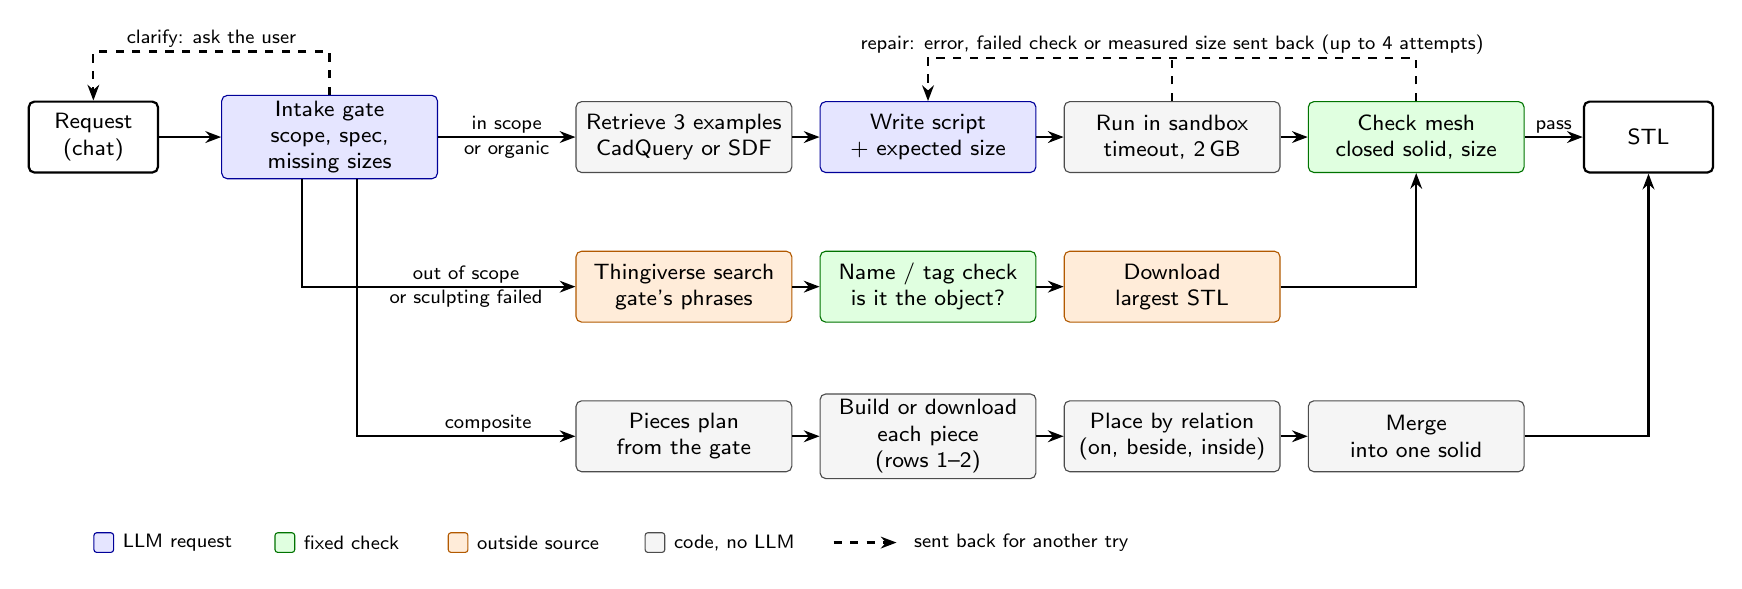
\begin{tikzpicture}[
    font=\sffamily\footnotesize,
    >={Stealth[length=2mm]},
    box/.style={draw, rounded corners=2pt, align=center, minimum height=9mm, text width=26mm, inner sep=2pt},
    llm/.style={box, fill=blue!10, draw=blue!60!black},
    check/.style={box, fill=green!12, draw=green!45!black},
    ext/.style={box, fill=orange!15, draw=orange!70!black},
    plain/.style={box, fill=gray!8, draw=gray!60!black},
    io/.style={box, text width=15mm, fill=white, draw=black, thick},
    lab/.style={font=\sffamily\scriptsize, align=center, inner sep=1pt},
    flow/.style={->, thick},
    back/.style={->, thick, dashed},
  ]
  % --- row 1: build with code (CadQuery, or SDF for organic shapes) ---
  \node[io]    (req)  at (0, 0)     {Request\\(chat)};
  \node[llm]   (gate) at (3.0, 0)  {Intake gate\\scope, spec, missing sizes};
  \node[plain] (ret)  at (7.5, 0)  {Retrieve 3 examples\\CadQuery or SDF};
  \node[llm]   (gen)  at (10.6, 0)  {Write script\\+ expected size};
  \node[plain] (run)  at (13.7, 0) {Run in sandbox\\timeout, 2\,GB};
  \node[check] (chk)  at (16.8, 0) {Check mesh\\closed solid, size};
  \node[io]    (stl)  at (19.75, 0)  {STL};

  \draw[flow] (req) -- (gate);
  \draw[flow] (gate) -- node[lab, above] {in scope} node[lab, below] {or organic} (ret);
  \draw[flow] (ret) -- (gen);
  \draw[flow] (gen) -- (run);
  \draw[flow] (run) -- (chk);
  \draw[flow] (chk) -- node[lab, above] {pass} (stl);

  % repair loop (above row 1)
  \draw[back] (chk.north) -- ++(0, 0.55) -| node[lab, pos=0.25, above]
    {repair: error, failed check or measured size sent back (up to 4 attempts)} (gen.north);
  \draw[thick, dashed] (run.north) -- ++(0, 0.55);
  % clarify loop (above row 1, left)
  \draw[back] (gate.north) -- ++(0, 0.55) -| node[lab, pos=0.25, above]
    {clarify: ask the user} (req.north);

  % --- row 2: download ---
  \node[ext]   (ts)   at (7.5, -1.9)  {Thingiverse search\\gate's phrases};
  \node[check] (tn)   at (10.6, -1.9)  {Name / tag check\\is it the object?};
  \node[ext]   (td)   at (13.7, -1.9) {Download\\largest STL};

  \draw[flow] (gate.south) ++(-0.35, 0) |- node[lab, pos=0.8, above] {out of scope}
    node[lab, pos=0.8, below] {or sculpting failed} (ts.west);
  \draw[flow] (ts) -- (tn);
  \draw[flow] (tn) -- (td);
  \draw[flow] (td.east) -| (chk.south);

  % --- row 3: combined parts ---
  \node[plain] (plan) at (7.5, -3.8)  {Pieces plan\\from the gate};
  \node[plain] (each) at (10.6, -3.8)  {Build or download\\each piece (rows 1--2)};
  \node[plain] (pl)   at (13.7, -3.8) {Place by relation\\(on, beside, inside)};
  \node[plain] (mg)   at (16.8, -3.8) {Merge\\into one solid};

  \draw[flow] (gate.south) ++(0.35, 0) |- node[lab, pos=0.8, above] {composite} (plan.west);
  \draw[flow] (plan) -- (each);
  \draw[flow] (each) -- (pl);
  \draw[flow] (pl) -- (mg);
  \draw[flow] (mg.east) -| (stl.south);

  % --- legend ---
  \begin{scope}[shift={(0, -5.15)}, every node/.style={font=\sffamily\scriptsize, anchor=west}]
    \node[draw=blue!60!black, fill=blue!10, minimum size=2.5mm, inner sep=0, rounded corners=1pt] (l1) at (0, 0) {};
    \node at (0.25, 0) {LLM request};
    \node[draw=green!45!black, fill=green!12, minimum size=2.5mm, inner sep=0, rounded corners=1pt] at (2.3, 0) {};
    \node at (2.55, 0) {fixed check};
    \node[draw=orange!70!black, fill=orange!15, minimum size=2.5mm, inner sep=0, rounded corners=1pt] at (4.5, 0) {};
    \node at (4.75, 0) {outside source};
    \node[draw=gray!60!black, fill=gray!8, minimum size=2.5mm, inner sep=0, rounded corners=1pt] at (7.0, 0) {};
    \node at (7.25, 0) {code, no LLM};
    \draw[back] (9.4, 0) -- (10.2, 0);
    \node at (10.3, 0) {sent back for another try};
  \end{scope}
\end{tikzpicture}
}
  \caption{Pipeline. The intake gate (one LLM request) reads the chat and either asks for missing sizes or routes
    the request. In-scope parts are written as CadQuery code with three retrieved examples; organic objects are
    sculpted with SDF code through the same loop. Each script runs in a sandbox and the mesh is checked (closed
    solid, size against the request); a failure is sent back for a repair, up to four attempts. Objects code can't
    build are searched on Thingiverse, and combined parts are built or downloaded piece by piece, placed and merged.}
  \label{fig:pipeline}
\end{figure*}

\subsection{Intake gate}
% One LLM request: scope, filled-in spec, unknown parameters (critical or not). Fixed rules choose proceed /
% clarify / out of scope; composite plans with pieces. Not evaluated in this round (say so; Sec. 6).
\TODO{gate}

\subsection{Retrieved examples}
% 26 hand-checked CadQuery examples (scripts/make_examples.py), each request plus generic shape keywords;
% TF-IDF retriever, top 3 into the prompt. History, one sentence: an embedding retriever, a similarity cutoff and
% an external Text-to-CadQuery pool were tried and dropped (no gain; retrieval-lib26.md, external-rag.md).
\TODO{RAG}

\subsection{Generate, run, check, repair}
% The model writes a script plus its own BBOX line (expected size). Sandbox: separate process, timeout, 2 GB cap.
% Checks: valid watertight mesh (trimesh), size matches the request. On failure the error goes back
% (script error, mesh check failed, size off with the measured size, #23; no code; reply cut off), up to 4 attempts.
\TODO{repair loop}

\subsection{Organic shapes: sculpting and Thingiverse}
% Out-of-scope objects with an organic_spec are sculpted: the model writes SDF code (fogleman/sdf API on our own
% small library, meshed with manifold3d level sets; 11 SDF examples retrieved); every shape is stood on z = 0
% (#47). Otherwise / as fallback: Thingiverse search, name/tag check that the result is the object (#39),
% download, validate.
\TODO{SDF sculpting; Thingiverse}

\subsection{Combined parts}
% Composite plans: base first, pieces generated or downloaded, scaled to height, placed (on_top / under / beside /
% inside) by bounding boxes, merged with manifold3d. Not benchmarked; one example figure at most.
\TODO{assembly}

\subsection{Local models and fine-tuning}
\label{sec:finetune}
% Ollama for fully local use (default gemma4:12b). Student: Qwen3.5-4B, 4-bit QLoRA (rank 16, 2 epochs) on 1,052
% teacher conversations (822 CadQuery, 230 SDF; 990 train / 62 validation; teachers Sonnet and
% gemini-3.5-flash-lite), kept only when the part was valid
% and the right size (SDF: judge pass too). Failed attempts and repairs kept in the conversations. Requests are
% filtered against benchmark cases. Source: finetune-v2.md (data/training only; results from report-v1.md).
\TODO{fine-tuned student}

\section{Evaluation}
\label{sec:evaluation}

% ~1.25 pages. Everything here is from report-v1.md (header, "Choosing the judge", "For writing the report") and
% eval/studies/report-v1.toml. Say early: one round, one code version, comparisons named before the runs.

\subsection{Benchmarks}
% Main suite: 48 requests (simple 5, medium 17, hard 13, proposal 8, casual 5); 42 should be built, 3 declined,
% 3 either. Each with an expected bounding box has a hand-written reference solution that builds at that size
% (eval/references.py), never shown to the model. None copied from the example library.
% Organic suite: 30 objects (animals, figures, ...), no expected size; no organic subject in the SDF examples.
% Appendix A lists every case.

The total benchmark was derived of 78 requests to the agent.
Form these 78 requests, 48 were mechanical parts and 30 were organic.
Each of the mechanical requests belonged to one of four categories: simple requests (5), medium-difficulty requests (17), hard-difficulty requests (13), and casual requests (13).
Casual requests are ones that do not follow a specific mechanical request, similar to organic style requests.
Each object in the casual was hand-checked as to whether the model should reject building the part, require building it, or allow either a rejection or build.

The organic suite is similar to the casual requests, except specifically focused on sculpting shapes.
For example, the 12th organic benchmark requests: "A turtle 60 mm long: a domed shell, four stubby legs, a head poking out the front and a short tail."

\subsection{Builders and configurations}
% Table 1: builders. Columns: model, where it runs (API / Google API / local RTX 3080), configs run.
%   claude-sonnet-5-5, claude-haiku-5-5, gemini-3.5-flash-lite, gemma-4-31b-it (Google API), gemma4:12b (local
%   default), qwen3.5:4b (local base), cad-qwen3.5:4b-v2 (fine-tuned), plus Thingiverse (organic only).
% Configs: rag-size (3 retrieved examples, measured-size message: the app's setup), norag-size (no examples),
% sdf (organic, 11 SDF examples), thingiverse-check (first matching download). 4 attempts max. 3 runs per pair.
% Gemma 31B, Haiku and the no-RAG Qwen arms were added during the round ("Changes during the round").
\TODO{text for Table 1}

% Table 1: from the round's rows (eval/results/studies/report-v1/, one arm per model, suite and config):
% 144 runs per main-suite arm (48 cases x 3), 90 per organic SDF arm (30 x 3), 30 Thingiverse runs; 2,118 in all.
\begin{table}[t]
  \centering
  \small
  \setlength{\tabcolsep}{3pt}
  \begin{tabular}{@{}llccc@{}}
    \toprule
    & & \multicolumn{2}{c}{Main suite} & Organic \\
    \cmidrule(lr){3-4} \cmidrule(l){5-5}
    Builder & Runs on & RAG & no RAG & SDF \\
    \midrule
    Claude Sonnet 5.5          & Anthropic     & \checkmark & \checkmark &            \\
    Claude Haiku 5.5           & Anthropic     & \checkmark & \checkmark & \checkmark \\
    Gemini 3.5 Flash Lite      & Google        & \checkmark & \checkmark & \checkmark \\
    Gemma 4 31B                & Google        & \checkmark &            &            \\
    Gemma 4 12B$^\dagger$      & local         & \checkmark &            &            \\
    Qwen3.5 4B fine-tuned      & local         & \checkmark & \checkmark & \checkmark \\
    Qwen3.5 4B (base)          & local         & \checkmark & \checkmark & \checkmark \\
    \midrule
    Thingiverse                & Thingiverse   & \multicolumn{2}{c}{--} & download \\
    \bottomrule
  \end{tabular}
  \caption{Builders and the configurations each was run with. \emph{RAG}: three retrieved examples in the prompt
    (the app's setup); \emph{no RAG}: none; \emph{SDF}: organic objects sculpted with SDF code and 11 SDF examples; Thingiverse
    search takes the first matching download instead. API models run on the provider's servers. Every model run allows up to 4 attempts and
    is repeated 3 times per case (Thingiverse once); 2,118 runs in all. Local models run in Ollama on one RTX 3080 (10\,GB). $^\dagger$The app's default local model.}
  \label{tab:builders}
\end{table}

\subsection{Metrics}
% Correct: built at the expected size (or declined when it should be); organic: a valid mesh.
% Right size + shape: correct and the visual judge passes it (organic: any part that came out and passes).
% Also: first-try rate, correct after k attempts, pass@k over the 3 repeats~\cite{chen2021codex},
% tokens, $ per correct part, time.
\TODO{metrics}

\subsection{Visual judge}
\label{sec:judge}
% Six views per part (front, right, top, bottom flat; two isometric), one request with the request text and the
% measured size; score 0-1 on four bands (match / minor / feature wrong / different object; top two pass).
% Choice: 4 judges x 204 items x 3 runs; items = 58 reference checks + 146 hand-graded parts (100 graded blind:
% no builder, config or judge score shown). Rule written before the runs: best held-out accuracy, the cheaper one
% if the interval overlaps the old judge's. It picks Sonnet; Sonnet for every part (~$5.90) was over the remaining
% budget, so gemini-3.8-flash (statistically tied, 92% vs 96%, p = 0.08) judges the main suite and Sonnet the
% organic suite, where gemini-3.8-flash is weak (71% vs 91%). State this deviation plainly. Results in Sec. 5.7.
\TODO{judge}

% Figure: renders copied by `pixi run -e cap6938 python -m scripts.report_figures judge-example`, which also prints
% the judge's replies quoted below (gemini-3.8-flash, report-v1, same verdict in all 3 runs).
\begin{figure*}[t]
  \centering
  \small
  \textit{``Can you make me something to stand my AA batteries up in? 8 of them in two rows of four, holes 15mm wide
    and 20mm deep, in an 80 x 40 x 25 block.''}\\[4pt]
  \begin{minipage}[t]{0.485\linewidth}
    \centering
    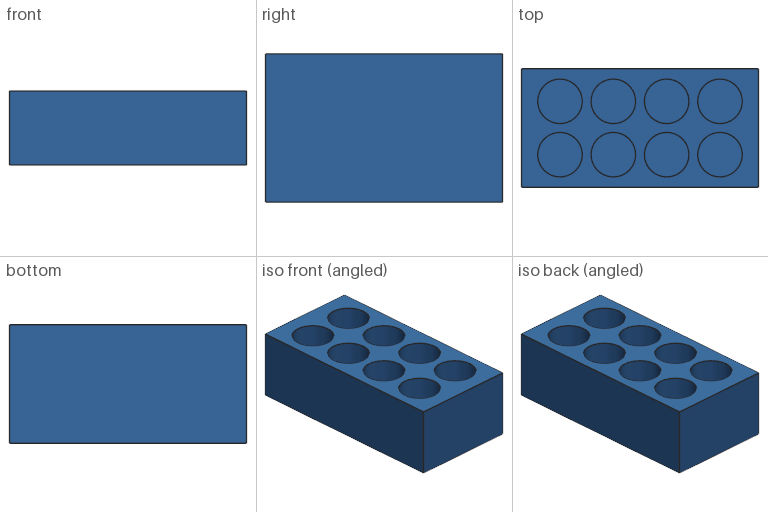
\includegraphics[width=\linewidth]{figures/judge_c01_reference.png}\\[2pt]
    (a) Reference solution: score 1.0 (\emph{pass}).
  \end{minipage}\hfill
  \begin{minipage}[t]{0.485\linewidth}
    \centering
    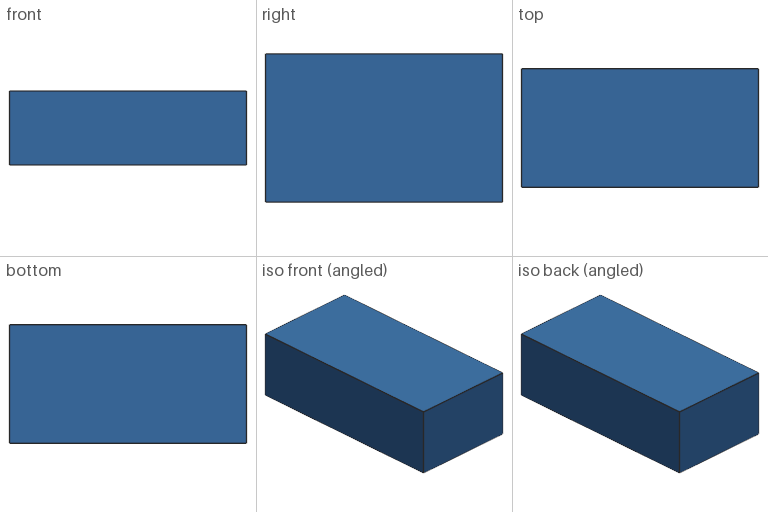
\includegraphics[width=\linewidth]{figures/judge_c01_gemma31b.png}\\[2pt]
    (b) Gemma 4 31B build: score 0.11 (\emph{fail}). ``Missing all 8 holes for the AA batteries; part is a
    completely solid block.''
  \end{minipage}
  \caption{What the visual judge sees: six views of the part (four flat, two angled), sent in one request with the
    request text and the measured size. Both parts measure $80 \times 40 \times 25$\,mm, so the size check accepts
    both; only the top and angled views show that (b) has no holes. The judge scores 1--10 on four bands (match,
    small deviations, a feature wrong, a different object), rescaled to 0--1; 0.5 and above passes. It gave each part
    the same score in all 3 runs, and the hand grade for (b) is ``different object''.}
  \label{fig:judge}
\end{figure*}

% Figure: made by `pixi run -e cap6938 python -m scripts.report_figures render-fix`. From development, before the
% report round: judge gemini-3.1-flash-lite, render/prompt v1 vs v2 (eval/results/judge-gemini-3.1-flash-lite.md).
\begin{figure}[t]
  \centering
  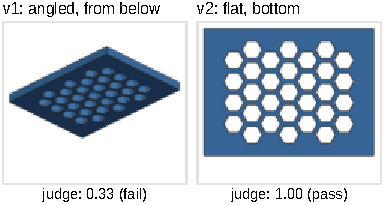
\includegraphics[width=\linewidth]{figures/render_fix.pdf}
  \caption{Why the renders include a flat bottom view. The reference solution for a honeycomb panel with hexagonal
    through-holes, seen from below in our first render version (left) and the current one (right). From the angled
    view the first judge, gemini-3.1-flash-lite, concluded ``the holes are not actual through-holes; they are
    recessed pockets'' and failed this correct part, although the flat top view already showed the background
    through the holes. With the flat bottom view, and a prompt line saying that only flat views show a through-hole as
    see-through, it passed. Fig.~\ref{fig:failures}b shows the reverse case: pockets that the flat bottom view exposes.}
  \label{fig:render-fix}
\end{figure}

\subsection{Statistics}
% Rate = mean over cases of each case's rate over 3 runs. 95% intervals: bootstrap over cases~\cite{efron1993bootstrap}
% (repeats are not independent). Comparisons paired by case: mean difference with interval and exact sign test.
% Judges: McNemar's exact test~\cite{mcnemar1947}, Cohen's kappa~\cite{cohen1960kappa}. Code: eval/stats.py.
% The compared pairs were written in the manifest before the runs.
\TODO{statistics}

\section{Results}
\label{sec:results}

% ~3 pages. Each subsection: the claim first, then the number with its interval / p, then the table or figure.
% Source for every number: eval/results/report-v1.md (table names in the comments).

\subsection{Which model builds the part (RQ1)}
\label{sec:res-models}
% Table 2 (report-v1 "Summary"): right size, right size + shape with intervals, per model (rag-size).
% Figure 2: right size + shape per model with 95% intervals (bar or dot plot).
% Sonnet 99% [96-100], Haiku 94% [89-99], Gemini Flash Lite 74% [64-84], gemma-4-31b-it 74% [65-83],
% gemma4:12b 55% [42-67], fine-tuned Qwen 30% [19-41], base Qwen 13% [6-22].
% Sonnet vs Gemini +24 pts [+14, +35], p < 0.001; Haiku vs Gemini +20 pts, p < 0.001 ("Comparisons").
% The main suite no longer separates the two Claude models (ceiling).
\TODO{model comparison}

\subsection{Retrieved examples (RQ2)}
\label{sec:res-rag}
% "Comparisons" table. No measurable effect for API models: Gemini 74% vs 74% (+1 pts [-8, +9]), Sonnet 99 vs 98,
% Haiku 94 vs 95. Fine-tuned 4B: right shape 30% vs 18% (+12 [+3, +21], p = 0.04), first try 28% vs 8%;
% it was trained with examples in every prompt, so this measures RAG and training format together.
% Base 4B: within noise (17% vs 10% correct, p = 0.18), but builds a valid part more often (12% vs 3%) and needs
% half the tokens per correct part. Examples do raise first-try rates for Gemini (55% -> 67%) and Haiku.
\TODO{RAG}

\subsection{Fine-tuning a small local model (RQ3)}
\label{sec:res-ft}
% Fine-tuned vs base Qwen 4B: right size 51% vs 17% (+34 [+22, +47], p < 0.001), right shape 30% vs 13%
% (p = 0.007), a third of the tokens per correct part ("Tokens and cost"). Still below gemma4:12b (-25 pts shape,
% p < 0.001). Organic: valid mesh 36% vs 3%, but right shape only 1%: it learned to produce SDF code that runs,
% not the shape.
\TODO{fine-tuning}

\subsection{Model size versus running locally}
\label{sec:res-size}
% Same Gemma 4 family: 31B on Google's servers vs 12B local: right shape 74% vs 55% (+19 [+6, +32], p = 0.005),
% right size +8 pts (p = 0.19, not significant). 31B matches Gemini Flash Lite. So the local gap is mostly size.
\TODO{size vs local}

\subsection{Repair loop and retries (RQ4)}
\label{sec:res-repair}
% Figure 3: correct after k = 1..4 attempts per model ("Repair loop and retries"), one line per model.
% Gemini 67% -> 88%, gemma4:12b 53% -> 77%, gemma-31b 52% -> 85%; Sonnet/Haiku 97% -> 99-100% (little to fix).
% Sculpting depends on it: Gemini 1% first try -> 82%, Haiku 26% -> 91%.
% Table 3 (maybe appendix): failure types and how often the next attempt fixed them; small Qwen almost never fixes
% a script error (base 1% of ~460).
% Retrying the whole request (pass@3): Gemini 88% -> 96%, fine-tuned Qwen 51% -> 73%, gemma4:12b 77% -> 88%.
\TODO{repair and retries}

\subsection{Organic shapes: sculpting or downloading (RQ5)}
\label{sec:res-organic}
% Judged by claude-sonnet-5-5. Right shape: Haiku 82% [71-92], Gemini 52% [40-64], Thingiverse 37% [20-53]
% (Gemini vs Thingiverse +16 pts, p = 0.33: not significant; Haiku vs Gemini +30, p = 0.001); small local models
% 0-1%. Thingiverse: a download came out for 67% of cases; many were the wrong object or a scene.
% Table 4 ("Organic suite under both judges"): gemini-3.8-flash rates Haiku's parts higher (90%), so the Claude
% judge does not favour Claude's parts.
% Figure 4: a few organic parts side by side (same case, Haiku / Gemini / Thingiverse) from eval/renders/.
\TODO{organic}

\subsection{How far the judge can be trusted}
\label{sec:res-judge}
% Table 5 ("Choosing the judge"): held-out accuracy, mechanical / organic, kappa vs grades, consistency, $/item.
% gemini-3.1-flash-lite 83%, gemini-3.8-flash 92%, Haiku 90%, Sonnet 96%.
% The old judge (used in all earlier studies) got 35 of 204 wrong and failed Claude-built parts 50 pts more often
% than the hand grades: earlier rounds understated strong models. No judge clearly favours its own family.
\TODO{judge reliability}

\subsection{Cost and time}
\label{sec:res-cost}
% Table 6 ("Tokens and cost", "Time"): $ per correct part and median build time.
% Haiku $0.0009, Gemini $0.0029, Sonnet $0.011 per correct part; Gemini fastest (median 3 s per build), Sonnet 6 s;
% gemma4:12b 136 s median (up to ~10 min), mostly thinking (11.5K output tokens per run). Total spend ("Spend").
\TODO{cost and time}

\section{Discussion}
\label{sec:discussion}

% ~1 page.

% Which knowledge helps whom (tie back to the four kinds in the intro):
%  - weights matter most: size and fine-tuning move results by 20-35 pts;
%  - execution feedback (repair) helps mid-strength models most and makes sculpting possible;
%  - retrieved examples help only models that need the format (fine-tuned student, base model's validity),
%    not models that already know CadQuery; history: rag-copying.md (#29) on whether examples get copied;
%  - an outside repository is a weak fallback for organic objects compared with sculpting by a strong model.
\TODO{what helped whom}

% Failure analysis: common failure types (size off, wrong feature, script errors in small models), with 2-3
% example renders (eval/renders/) of typical mistakes. Organic: blobby or missing parts; Thingiverse: wrong object.
\TODO{failure analysis}

% Limitations (report-v1.md "Caveats"): 48 + 30 cases; one human grader, only 34 graded organic parts;
% main suite at ceiling for Claude models; judge choice departed from the pre-set rule (budget); token counts only
% comparable within a family; local timing on one RTX 3080.
\TODO{limitations}

% Not measured (report-v1.md "For writing the report"): the intake gate and the whole app path (#12), combined
% parts (#10), harder cases, a second grader, gemma4:12b and Sonnet on the organic suite.
\TODO{not measured}

\section{Conclusion}
\label{sec:conclusion}

% One line per research question, then 2-3 sentences of future work:
%  RQ1 strong API models are near the ceiling; local gap is mostly size.  RQ2 examples help only weak/trained models.
%  RQ3 fine-tuning triples a 4B model's right-size rate, still behind 12B.  RQ4 repair adds ~20 pts for mid models.
%  RQ5 sculpting with a strong model beats downloading.
% Future work: harder benchmark, gate evaluation (#12), judge inside the build loop (#35), editing parts (#36),
% letting the gate choose sculpting or a download per piece (#55, e.g. download Spider-Man, sculpt the tree).
\TODO{conclusion}

\section*{AI usage statement}
\label{sec:ai-usage}

The codebase for this project was built primarily with the assistance of Claude Code, Anthropic's AI coding agent.
For this report, Claude Code was used for formatting, grammatical fixes and the outline.
Separately, Claude models are among the builders and judges evaluated in Sec.~\ref{sec:evaluation}.

{
    \small
    \nocite{*} % outline stage: list every entry; remove once the text cites them
    \bibliographystyle{ieeenat_fullname}
    \bibliography{main}
}

\clearpage
\appendix
\section{Appendix}
\label{sec:appendix}

% Not counted in the 8 pages.

% A. Benchmark cases: table of the 48 main cases (id, category, request, expected size) and the 30 organic cases
%    (id, subject, request). From eval/cases.json and eval/organic_cases.json.
\TODO{case lists}

% B. Prompts: build prompt (generate.py SYSTEM_PROMPT), SDF prompt (SYSTEM_PROMPT_SDF, maybe shortened), judge
%    prompt (judge/prompts/<version>.txt).
\TODO{prompts}

% C. Per-category results (report-v1.md "Per model and category"), full results table, failure-type table,
%    pass@k table, time table if not in the main text.
\TODO{extra tables}

% D. More renders: a sheet of example parts per model, good and bad.
\TODO{example renders}

% E. Spend and hardware (report-v1.md "Spend"; study header).
\TODO{spend}


\end{document}
